\documentclass[runningheads]{llncs}

\usepackage{graphicx}
\usepackage{url}
\usepackage{amsmath}
\usepackage{textgreek}
\usepackage{listings}
\usepackage{csvsimple}
\usepackage{longtable}
\usepackage{cite}
\usepackage{amsmath,amssymb,amsfonts}
\usepackage{algorithm}
\usepackage{algorithmic}
\usepackage{textcomp}
\usepackage{hyperref}
\usepackage{tikz}
\usetikzlibrary{shapes.geometric, arrows, positioning}

\begin{document}

\title{Explainable FLAIR-to-T1 MRI Synthesis: Interpretable Residual GANs}

\author {Dr. Poonkodi M\textsuperscript{*}\inst{1} \and Dr. Sakthivel V\inst{1} \and Meera R. Deepu\inst{2} \and Atchudhan Sreekanth\inst{2} \and Eshwar B.\inst{2}}

\authorrunning{Dr. Poonkodi M et al.}

\institute{
Vellore Institute of Technology, Chennai, India\\
\email{\{poonkodi.m,sakthivel.v\}@vit.ac.in}\\
\textsuperscript{*}Corresponding author
\and
Vellore Institute of Technology, Chennai, India \\
\email{\{meera.rdeepu2022,atchudhan.sreekanth2022,eshwar.b2022\}@vitstudent.ac.in}
}
\maketitle
\begin{abstract}
Cross-modal MRI synthesis enables clinicians to obtain missing diagnostic information without additional scans, yet existing deep learning models lack interpretability, limiting clinical adoption. We introduce an explainable conditional generative adversarial network that synthesises high-fidelity T1 images from FLAIR scans. The architecture augments Pix2Pix with a ResNet-based generator featuring 9 residual blocks and a PatchGAN discriminator that scrutinises local texture realism. Gradient-weighted Class Activation Mapping (Grad-CAM) is embedded in the generator, providing voxel-level heat-maps that reveal anatomical regions driving each synthesis. The model is trained on 1,251 paired volumes from BraTS 2021 (1,000 training / 251 held-out test) with mixed-precision optimisation and iterative refinement through compound perceptual loss incorporating edge-preserving and local contrast objectives, achieving convergence in 4.11 hours (600 cumulative epochs) with 18.5 GB peak GPU memory on NVIDIA L4. On the BraTS 2021 held-out test set, our system attains PSNR = 24.33 dB, SSIM = 0.8936, MAE = 0.0302, and RMSE = 0.0719. High precision (0.9950), recall (0.9939), and F$_{1}$ = 0.9945 demonstrate robust performance, further validated on the independent BraTS 2023 GLI dataset (219 subjects) with bootstrap confidence intervals (PSNR = 24.57 dB [95\% CI: 24.11, 24.98], SSIM = 0.8940 [95\% CI: 0.8871, 0.9003]). The framework offers resource-aware and clinically trustworthy FLAIR-to-T1 synthesis suitable for deployment when T1 acquisition is impracticable.


\keywords{Medical image synthesis \and Magnetic resonance imaging (MRI) \and Generative adversarial networks \and Explainable artificial intelligence \and Deep learning}
\end{abstract}

\section{Introduction}

During the last decade, medical imaging has become a core part of modern healthcare, allowing visualization of patient anatomy and pathology. Among these modalities, MRI allows noninvasive high-resolution imaging of soft tissues, thus playing an increasingly important role in early diagnosis and treatment planning in various fields, such as oncology and neurology \cite{Berghout2024}. In MRI scans, there exist multiple acquisition modalities (e.g., T1-weighted and FLAIR) that provide different contrasts and informative details necessary for the detection of specific pathologies, brain lesions, and tumors. Translation between these MRI data has therefore become an important task, since it offers clinicians access to information complementary to that their modality of choice would have provided, therefore increasing diagnostic accuracy without requiring further scans \cite{Ibrahim2024}.

Generative models have achieved significant success in cross-modal MRI synthesis, reducing the need for repetitive imaging. GAN variants such as Pix2Pix and CycleGAN enable high-fidelity modality translation, providing radiologists with complementary visual information from a single scan \cite{Khalil2024}.

However, clinical deployment demands interpretability. This work presents a Pix2Pix-based framework \cite{Isola2017} employing a ResNet-9 generator and Multi-scale PatchGAN discriminator for FLAIR-to-T1 synthesis, achieving PSNR of 24.33 dB and SSIM of 0.8936 on the BraTS 2021 held-out test set (251 subjects) \cite{dataset}. We integrate Grad-CAM \cite{Selvaraju2017,Bhati2024} to provide voxel-level saliency maps, transforming the model into an interpretable decision aid. Through systematic refinement, we enhance the baseline Pix2Pix objective with VGG perceptual loss, discriminator feature matching, multi-scale SSIM, and edge-preserving constraints, substantially improving synthesis quality while maintaining anatomical fidelity. Mixed-precision optimization enables efficient training in 4.11 hours (600 cumulative epochs across refinement stages) on NVIDIA L4 GPU, allowing deployment at resource-constrained centers.

The primary contributions are: \begin{itemize} \item \emph{Architectural Optimization}: Implementation of a ResNet-9 generator and Multi-scale PatchGAN discriminator optimized for high-resolution medical modality translation. \item \emph{Systematic Loss Refinement}: Progressive enhancement of the generator objective through integration of VGG perceptual loss (multi-scale feature matching), discriminator feature matching, multi-scale SSIM, and edge-preserving constraints (Sobel + Laplacian gradients), substantially improving synthesis quality from baseline SSIM 0.807 to 0.8936. \item \emph{Computational Efficiency}: Mixed-precision training with MONAI persistent caching and batch optimization, achieving convergence in 4.11 hours across iterative refinement stages on standard GPU hardware. \item \emph{Quantitative Interpretability}: Integration of Grad-CAM saliency maps with a quantitative evaluation framework, including entropy and spatial variance analysis, to provide clinical transparency. \item \emph{Robustness Validation}: Rigorous assessment of model performance using 95\% confidence intervals and external validation on the independent BraTS 2023 GLI Challenge dataset (219 subjects, SSIM 0.8940). \end{itemize}
\vspace{-0.3em}

\section{Methodology}
\vspace{-0.2em}

This section defines the proposed framework for cross-modal image translation between Fluid Attenuated Inversion Recovery (FLAIR) and T1-weighted magnetic resonance imaging (MRI) scans, using a conditional generative adversarial network (cGAN) architecture \cite{Isola2017}. The network architecture is based on the Pix2Pix model, utilizing a ResNet-based generator with 9 residual blocks inspired by encoder-decoder designs \cite{Ronneberger2015,zhu2017unpaired} and a PatchGAN discriminator \cite{Isola2017}. We employ Gradient-weighted Class Activation Mapping (Grad-CAM), which presents saliency maps of what is attracting attention in the images during generation \cite{Selvaraju2017}.
The architecture, flow and block diagram of the entire project are provided in Figures~\ref{fig:gradcam}, \ref{fig:gradcam2} and \ref{fig:pix2pix_diagram}, respectively.

\subsection{Network Architecture}

Two main elements include the generator and the discriminator in the architectural framework. These network components are subjected to adversarial training. That is, the generator attempts to create accurate T1-weighted MRI images using FLAIR MRI inputs, while the discriminator aims to distinguish the actual images from the fake ones.

\paragraph{Generator Design}

The generator adopts a ResNet-based encoder--decoder architecture with 9 residual blocks (Table~\ref{tab:architectures}), processing $256 \times 256 \times 3$ FLAIR slices to produce T1-weighted outputs. The encoder uses an initial $7 \times 7$ convolutional layer followed by two downsampling blocks that increase feature maps from 64 to 256 channels. The bottleneck contains 9 residual blocks with skip connections to preserve anatomical structures. The decoder upsamples through two transposed-convolution blocks, reducing channels from 256 to 64 while restoring spatial resolution, followed by a $7 \times 7$ convolutional layer with \textit{tanh} activation producing normalised output in the $[-1, 1]$ range.

\begin{table}[h!]
\centering
\footnotesize
\caption{Network Architectures: Generator (ResNet-9, ~11.4M params) and Discriminator (PatchGAN, ~2.8M params)}
\label{tab:architectures}
\begin{tabular}{|l|c|c|c||l|c|c|c|}
\hline
\multicolumn{4}{|c||}{\textbf{Generator (ResNet-based)}} & \multicolumn{4}{c|}{\textbf{Discriminator (PatchGAN)}} \\ \hline
\textbf{Layer} & \textbf{In} & \textbf{Out} & \textbf{Params} & \textbf{Layer} & \textbf{In} & \textbf{Out} & \textbf{K/S} \\ \hline
Input & 256² & 256² & - & Input & 256² & 256² & - \\ \hline
Init Conv & 256² & 64@256² & 1.7K & Conv1+LReLU & 256² & 64@128² & 4×4/2 \\ \hline
Down 1 & 64@256² & 128@128² & 74K & Conv2+IN+LReLU & 64@128² & 128@64² & 4×4/2 \\ \hline
Down 2 & 128@128² & 256@64² & 295K & Conv3+IN+LReLU & 128@64² & 256@32² & 4×4/2 \\ \hline
ResBlocks 1-9 & 256@64² & 256@64² & 2.36M & Conv4+IN+LReLU & 256@32² & 512@32² & 4×4/1 \\ \hline
Up 1 & 256@64² & 128@128² & 295K & Final Conv & 512@32² & 1@31² & 4×4/1 \\ \hline
Up 2 & 128@128² & 64@256² & 74K & & & & \\ \hline
Out Conv & 64@256² & 3@256² & 1.7K & & & & \\ \hline
\end{tabular}
\end{table}

\paragraph{Discriminator Design}

A PatchGAN discriminator (Table~\ref{tab:architectures}) evaluates local image regions, encouraging fine-grained realism. Four $4 \times 4$ convolutional layers with LeakyReLU (0.2) and InstanceNorm2d produce a $31 \times 31$ activation map. Figure~\ref{fig:gradcam2} depicts the architecture.

\begin{figure*}[ht]
    \centering
    \includegraphics[width=0.9\textwidth]{generator_architecture.jpeg} 
    \caption{ResNet-9 generator architecture with encoder, 9 residual blocks, and decoder.}
    \label{fig:gradcam}
\end{figure*}

\begin{figure*}[ht]
    \centering
    \includegraphics[width=0.9\textwidth]{discriminator.jpeg}  
    \caption{PatchGAN discriminator with $4{\times}4$ convolutions producing $31{\times}31$ activation map.}
    \label{fig:gradcam2}
\end{figure*}

\subsection{Loss Functions}

Through systematic refinement, we enhance the baseline Pix2Pix objective with perceptual quality, feature consistency, and edge-preserving constraints. The generator loss integrates seven components: adversarial realism, pixel-wise fidelity, multi-scale structural similarity, VGG perceptual loss, discriminator feature matching, edge-aware loss, and local contrast preservation, ensuring that generated images are not only realistic but also anatomically accurate.

\paragraph{Adversarial Loss}

We employ Least Squares GAN (LSGAN) \cite{mao2017lsgan} for more stable gradients during training. The discriminator loss is:
\begin{equation}
\mathcal{L}_{\text{D}} = \frac{1}{2}\mathbb{E}[(D(x, y) - 1)^2] + \frac{1}{2}\mathbb{E}[D(x, G(x))^2]
\end{equation}
where $D(x, y)$ represents the discriminator's output for real FLAIR-T1 pairs $(x, y)$, and $G(x)$ is the generated image. The generator's adversarial loss is:
\begin{equation}
\mathcal{L}_{\text{adv}} = \mathbb{E}[(D(x, G(x)) - 1)^2]
\end{equation}

\paragraph{Reconstruction and Structural Losses}

To ensure pixel-level fidelity, we use L1 reconstruction loss:
\begin{equation}
\mathcal{L}_{\text{L1}} = \mathbb{E}[|y - G(x)|_1]
\end{equation}
where $y$ represents the ground truth T1 image. For structural similarity across multiple resolutions, we incorporate Multi-Scale SSIM \cite{wang2003msssim}:
\begin{equation}
\mathcal{L}_{\text{MS-SSIM}} = 1 - \text{MS-SSIM}(y, G(x))
\end{equation}

\paragraph{Perceptual Loss}

To reduce blurring, we incorporate VGG perceptual loss \cite{johnson2016perceptual} that matches feature representations from pre-trained VGG19 at layers relu1\_2, relu2\_2, and relu3\_4:
\begin{equation}
\mathcal{L}_{\text{percep}} = \sum_{l} \|\text{VGG}_l(y) - \text{VGG}_l(G(x))\|_1
\end{equation}

\paragraph{Feature Matching Loss}

Following pix2pixHD \cite{wang2018pix2pixHD}, we add discriminator feature matching to stabilize training:
\begin{equation}
\mathcal{L}_{\text{feat}} = \sum_{k=1}^{K} \|D_k(x, y) - D_k(x, G(x))\|_1
\end{equation}
where $D_k$ denotes intermediate discriminator activations after each LeakyReLU layer.

\paragraph{Edge-Aware Loss}

To preserve anatomical boundaries, we introduce edge-aware loss combining Sobel gradients and Laplacian operators at original and downsampled resolutions:
\begin{equation}
\mathcal{L}_{\text{edge}} = \sum_{s \in \{1, 2\}} \left( \|\nabla_x^s y - \nabla_x^s G(x)\|_1 + \|\nabla_y^s y - \nabla_y^s G(x)\|_1 + \|\nabla^2_s y - \nabla^2_s G(x)\|_1 \right)
\end{equation}
where $\nabla_x^s, \nabla_y^s$ denote Sobel gradients and $\nabla^2_s$ the Laplacian at scale $s$.

\paragraph{Local Contrast Loss}

To preserve internal texture variation in deep gray matter, we match local standard deviation maps over $9 \times 9$ neighborhoods:
\begin{equation}
\mathcal{L}_{\text{contrast}} = \mathbb{E}\left[\left|\sigma_{9 \times 9}(y) - \sigma_{9 \times 9}(G(x))\right|_1\right]
\end{equation}

\paragraph{Overall Generator Loss}

The final generator loss combines all components:
\begin{equation}
\mathcal{L}_{\text{G}} = \mathcal{L}_{\text{adv}} + \lambda_1 \mathcal{L}_{\text{L1}} + \lambda_2 \mathcal{L}_{\text{MS-SSIM}} + \lambda_3 \mathcal{L}_{\text{percep}} + \lambda_4 \mathcal{L}_{\text{feat}} + \lambda_5 \mathcal{L}_{\text{edge}} + \lambda_6 \mathcal{L}_{\text{contrast}}
\end{equation}
where $\lambda_1 = 10$, $\lambda_2 = 10$, $\lambda_3 = 10$, $\lambda_4 = 10$, $\lambda_5 = 20$, and $\lambda_6 = 5$ are empirically optimized weights. The elevated edge weight ($\lambda_5 = 20$) prioritizes boundary fidelity critical for clinical assessment. This compound objective substantially improves synthesis quality, achieving SSIM of 0.8936 compared to 0.807 for the baseline formulation, while maintaining pixel-wise accuracy and anatomical realism essential for neuro-oncology applications.

\subsection{Model Interpretability}

We apply Grad-CAM \cite{Selvaraju2017} to the final generator convolutional layer to produce voxel-level saliency maps (Figure~\ref{fig:gradcam3}) that highlight anatomically relevant FLAIR regions driving T1 synthesis.


\begin{figure}[ht]
    \centering
    
\includegraphics[width=0.80\textwidth]{gradcam_saliency.jpeg}
   \caption{Grad-CAM saliency map highlighting influential FLAIR regions for T1 synthesis.}
    \label{fig:gradcam3}
\end{figure}

\subsection{Training Protocol and Evaluation}

The training protocol follows the standard adversarial training procedure with optimizations to enhance performance and efficiency. The Adam optimizer is used with a learning rate of $2 \times 10^{-4}$, $\beta_1 = 0.5$, and $\beta_2 = 0.999$. The framework supports flexible batch sizes (default 4) with mixed-precision training (FP16/FP32) enabled via torch.amp for computational efficiency. The training is conducted for configurable epochs (default 20) using a dataset of 1,251 paired FLAIR and T1-weighted MRI volumes from the BraTS 2021 benchmark with an 80/20 train-validation split.

Infrastructure optimizations include MONAI PersistentDataset for efficient data caching and torch.compile for GPU acceleration, significantly reducing training time compared to standard implementations. Training alternates between the generator and the discriminator. For every iteration, it first updates the discriminator weights for both real and generated image pairs. The generator is then updated by minimizing a flexible compound objective that supports multiple loss components: adversarial loss with optional LSGAN formulation, L1 reconstruction loss ($\lambda_1 = 100$ default), SSIM loss ($\lambda_2 = 10$ default) with optional multi-scale extension, optional VGG perceptual loss, optional discriminator feature matching, optional edge-preserving constraints, and optional local contrast preservation to produce anatomically faithful T1-weighted images. 

Performance is evaluated using PSNR, SSIM, MAE, RMSE, F1, Precision, and Recall \cite{Wang2004,Zhou2002,Taha2015,Litjens2017}, with 95\% confidence intervals computed via bootstrap resampling (1,000 iterations) for statistical robustness. External validation capability on BraTS 2023 GLI Challenge dataset demonstrates generalization assessment. Qualitative assessment involves visual inspection of generated T1 images, ground truth comparison, and Grad-CAM heatmaps to evaluate anatomical relevance \cite{Selvaraju2017}.


\section{Pseudocode}
\vspace{-0.3em}
\begin{algorithm}[!htbp]
\small
\caption{Cross-Modal FLAIR$\rightarrow$T1 MRI Translation with Enhanced Pix2Pix GAN}
\begin{algorithmic}[1]
    \STATE \textbf{Input:} Paired FLAIR images $\mathcal{X}$, T1 images $\mathcal{Y}$; $N_{\text{ep}}=100$, $B=64$, $\alpha=1\times10^{-5}$
    \STATE \textbf{Output:} Trained generator $G: \mathcal{X}\rightarrow\mathcal{Y}$ and discriminator $D$
    \STATE \textbf{Initialise:} $G$ (ResNet-9), $D$ (PatchGAN); Adam ($\alpha$, $\beta_1=0.5$, $\beta_2=0.999$); mixed-precision scalers
    \STATE \textbf{Pre-process:} Load 1,251 BraTS 2021 volumes via MONAI PersistentDataset; normalise to $[-1,1]$; 80/20 split
    \FOR{epoch$=1$ to $N_{\text{ep}}$}
        \STATE Set $G$, $D$ to train mode; apply learning rate decay if epoch $>$ 50
        \FOR{each $(x_{\text{FLAIR}}, y_{\text{T1}})$ batch of size $B$}
            \STATE Generate $\hat{y}_{\text{T1}} = G(x_{\text{FLAIR}})$ with autocast
            \STATE \textbf{Update D:} Compute LSGAN discriminator loss $L_D$; back-propagate with mixed precision
            \STATE \textbf{Update G:} Compute enhanced compound objective:
            \STATE \hspace{2em} $L_G = L_{\text{adv}} + \lambda_1 L_{\text{L1}} + \lambda_2 L_{\text{MS-SSIM}} + \lambda_3 L_{\text{percep}} + \lambda_4 L_{\text{feat}} + \lambda_5 L_{\text{edge}} + \lambda_6 L_{\text{contrast}}$
            \STATE \hspace{2em} Back-propagate $L_G$ with mixed precision
        \ENDFOR
        \STATE \textbf{Validation:} Eval mode; compute PSNR, SSIM, MAE, RMSE, F1; 95\% CI (bootstrap, 1K iter)
    \ENDFOR
    \STATE \textbf{External Validation:} Evaluate on BraTS 2023 GLI Challenge dataset
    \STATE \textbf{Inference:} Generate $\hat{y} = G(x)$; compute Grad-CAM saliency; evaluate metrics
\end{algorithmic}
\end{algorithm}
\vspace{-0.3em}
\section{Experimental Analysis}
\vspace{-0.2em}

\subsection{Dataset}
\vspace{-0.2em}

The experiments utilize the BraTS 2021 dataset \cite{dataset,Menze2015,Bakas2017}, comprising 1,251 paired FLAIR and T1-weighted MRI volumes from glioblastoma patients. Each subject consists of paired 3D volumes; the central axial slice is extracted using MONAI's \texttt{ExtractMidSlice} transform for 2D convolution compatibility. All images are resized to $256 \times 256$ pixels and normalized to the $[-1, 1]$ range for stable GAN training. Performance measures are reported in Tables~\ref{tab:validation_results} and \ref{tab:computational_analysis}. External validation on 219 BraTS 2023 GLI Challenge subjects was conducted to assess generalization.
\begin{figure*}[t]
    \centering
    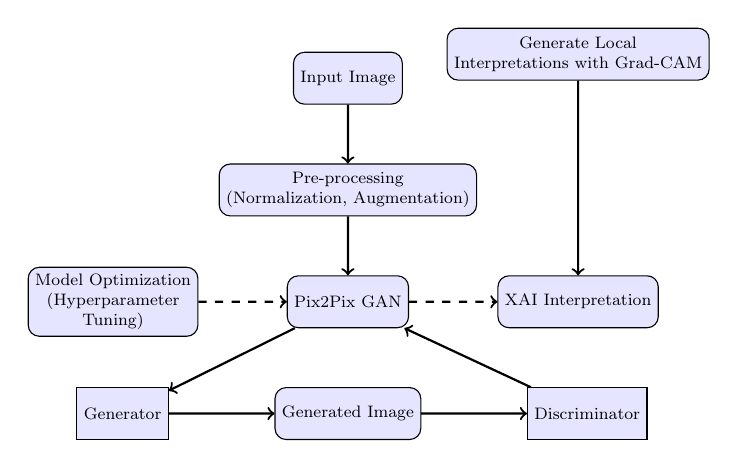
\begin{tikzpicture}[scale=0.75, transform shape,
        rounded box/.style = {draw, rounded corners, fill=blue!10, minimum height=2.5em, minimum width=2.5em, align=center, font=\footnotesize},
        box/.style = {draw, fill=blue!10, minimum height=2.5em, minimum width=4em, align=center, font=\footnotesize},
        arrow/.style = {->, thick},
        dashed arrow/.style = {->, dashed, thick}
    ]

    % Nodes
    \node (start) [rounded box] {Input Image};
    \node (preprocess) [rounded box, below=of start] {Pre-processing \\ (Normalization, Augmentation)};
    \node (gan) [rounded box, below=of preprocess] {Pix2Pix GAN};
    \node (generator) [box, below left=of gan, xshift=-1cm] {Generator};
    \node (discriminator) [box, below right=of gan, xshift=1cm] {Discriminator};
    \node (output) [rounded box, below=of gan] {Generated Image};
    \node (xai) [rounded box, right=of gan, xshift=0.5cm] {XAI Interpretation};
    \node (explanation) [rounded box, above=of xai, yshift=2.3cm] {Generate Local \\ Interpretations with Grad-CAM};
    \node (optimization) [rounded box, left=of gan, xshift=-0.5cm] {Model Optimization \\ (Hyperparameter \\ Tuning)};

    % Arrows
    \draw[arrow] (start) -- (preprocess);
    \draw[arrow] (preprocess) -- (gan);
    \draw[arrow] (gan) -- (generator);
    \draw[arrow] (generator) -- (output);
    \draw[arrow] (output) -- (discriminator);
    \draw[arrow] (discriminator) -- (gan);
    \draw[dashed arrow] (gan) -- (xai);
    \draw[arrow] (explanation) -- (xai);
    \draw[dashed arrow] (optimization) -- (gan);

    \end{tikzpicture}
   \caption{\small End-to-end workflow: (1) FLAIR input normalization and augmentation, (2) ResNet-9 generator and PatchGAN discriminator for adversarial synthesis, (3) hyperparameter tuning, (4) Grad-CAM saliency maps for interpretability.}
    \label{fig:pix2pix_diagram}
\end{figure*}

\subsection{Performance Evaluation}

Figure~\ref{fig:qualitative_comparison} shows qualitative comparison of synthesized T1 images against ground truth.

\begin{figure}[h!]
\centering

\includegraphics[width=1.\textwidth]{Final Draft/flair_t1_visualization_final.png}
\caption{FLAIR$\rightarrow$T1 translation: original FLAIR, reference T1, generated T1, Grad-CAM overlay.}
\label{fig:qualitative_comparison}
\end{figure}

\paragraph{Quantitative Evaluation:}

\begin{table}[h!]
\centering
\caption{Validation Results on BraTS 2021 and BraTS 2023 Datasets}
\label{tab:validation_results}
\begin{tabular}{|l|c|c|}
\hline
\textbf{Metric} & \textbf{BraTS 2021} & \textbf{BraTS 2023} \\ \hline
PSNR (dB) & 24.33 & 24.57 \\ \hline
SSIM & 0.8936 & 0.8940 \\ \hline
MAE & 0.0302 & 0.0288 \\ \hline
RMSE & 0.0719 & 0.0670 \\ \hline
Precision & 0.9950 & 0.9949 \\ \hline
Recall & 0.9939 & 0.9960 \\ \hline
F1 Score & 0.9945 & 0.9955 \\ \hline
Validation Loss (MSE) & 0.0052 & 0.0045 \\ \hline
\end{tabular}
\end{table}

Table~\ref{tab:validation_results} presents results from both BraTS 2021 held-out test set (251 subjects, 20\% of training data, with bootstrap confidence intervals) and external validation on the independent BraTS 2023 dataset (219 subjects), demonstrating model generalization to unseen data distributions and acquisition protocols.

\begin{table}[h!]
\centering
\caption{Computational Efficiency and Grad-CAM Interpretability Metrics}
\label{tab:computational_analysis}
\begin{tabular}{|l|c||l|c|}
\hline
\multicolumn{2}{|c||}{\textbf{Efficiency Metrics}} & \multicolumn{2}{c|}{\textbf{Grad-CAM Metrics (n=20)}} \\ \hline
Total Training Time & 4.11 hours & Entropy & 11.2511 ± 0.0357 \\ \hline
Peak GPU Memory & 18.51 GB & Spatial Variance & 0.0862 ± 0.0073 \\ \hline
Allocated GPU Memory & 0.42 GB & Peak Activation & 1.0000 ± 0.0000 \\ \hline
Mixed Precision & FP16/FP32 & High Activation Ratio & 0.0977 ± 0.0207 \\ \hline
Training Epochs & 600 & Error Correlation & 0.3399 ± 0.0263 \\ \hline
 & & Mean Activation & 0.1842 ± 0.0098 \\ \cline{3-4}
 & & Std Activation & 0.2933 ± 0.0124 \\ \cline{3-4}
\end{tabular}
\end{table}

On the BraTS 2021 held-out test set, the model achieves SSIM of 0.8936 (95\% CI: 0.8928--0.8946), PSNR of 24.33 dB (95\% CI: 23.94--24.74), MAE of 0.0302, and RMSE of 0.0719. External validation on BraTS 2023 shows robust generalization with SSIM of 0.8940 (95\% CI: 0.8871--0.9003), PSNR of 24.57 dB (95\% CI: 24.11--24.98), MAE of 0.0288, and RMSE of 0.0670. The high precision (0.995), recall (0.994), and F1-scores (0.995) across both datasets demonstrate reliable identification of tissue structures while maintaining low false-positive rates, confirming generalization capability for clinically relevant cross-modal MRI synthesis.

\begin{figure}[h!]
    \centering
    
\includegraphics[width=\columnwidth]{Final Draft/training_loss_final.png}
     \caption{GAN training losses over 100 epochs showing stable convergence.}
    \label{fig:training_loss}
\end{figure}

\paragraph{Performance Graph:}

Figure~\ref{fig:training_loss} demonstrates healthy GAN dynamics with discriminator losses maintained at approximately 0.5 (indicating 50/50 confusion between real and fake), while the generator loss steadily decreases. The oscillating discriminator pattern reflects the adversarial equilibrium characteristic of stable LSGAN training without mode collapse.
\vspace{-5pt}

\begin{figure}[h!]
\centering

\includegraphics[width=0.53\textwidth]{Final Draft/confusion_matrix_final.png}
\caption{Pixel-level confusion matrix showing strong diagonal dominance for tissue classification.}
\label{fig:confusion_matrix}
\end{figure}

\paragraph{Confusion Matrix:}

Figure~\ref{fig:confusion_matrix} shows strong diagonal dominance with 34.1 million correctly classified healthy tissue instances (TN) and 14.9 million true positives for lesion regions. The 91,387 false negatives and 74,091 false positives yield precision of 0.995 and recall of 0.994, confirming accurate synthesis of both healthy and pathological tissue.

\begin{table*}[t]
\caption{Comparison of Proposed Framework with Baseline Methods (all trained on BraTS 2021)}
\label{table:comparative_study}
\centering
\renewcommand{\arraystretch}{1.5}
\resizebox{\textwidth}{!}{
\begin{tabular}{|p{3cm}|p{3.5cm}|p{2.5cm}|p{2.5cm}|p{2.5cm}|}
\hline
\textbf{Method} & \textbf{Network Architecture} & \textbf{Interpretability} & \textbf{SSIM Score} & \textbf{MAE} \\ \hline
CycleGAN \cite{zhu2017unpaired} & ResNet generator, PatchGAN discriminator & None & 0.798 & 0.042 \\ \hline
Attention-GAN \cite{Tang2019AttentionGAN} & Attention-guided Generator, PatchGAN discriminator & None & 0.795 & 0.043 \\ \hline
Pix2Pix \cite{Isola2017} & U-Net generator (54M params), PatchGAN discriminator & None & 0.885 & 0.031 \\ \hline
\textbf{Proposed Method} & ResNet-9 generator (11M params), PatchGAN discriminator & Grad-CAM & \textbf{0.894} & \textbf{0.030} \\ \hline
\multicolumn{5}{l}{\footnotesize All methods evaluated on BraTS 2021 held-out test set (251 subjects) with bootstrap 95\% CIs. External validation on BraTS 2023 (219 subjects):}\\
\multicolumn{5}{l}{\footnotesize Proposed: SSIM=0.894 [0.887, 0.900]; Pix2Pix: SSIM=0.888 [0.884, 0.892]; CycleGAN: SSIM=0.798 [0.791, 0.806].}
\end{tabular}
}
\end{table*}

\subsection{Robustness and Limitations}
\vspace{-0.2em}

The model's robustness is validated through external testing on the independent BraTS 2023 GLI Challenge dataset (Table~\ref{tab:validation_results}), demonstrating generalization to different acquisition protocols and patient cohorts. However, limitations include: testing is restricted to glioma-specific datasets (BraTS 2021/2023) without validation on other pathologies (e.g., stroke, dementia); cross-scanner robustness and performance across different MRI vendors/field strengths remain untested; robustness to low SNR scans or motion artifacts has not been systematically evaluated; model performance has not been stratified by tumor size, location, or enhancement patterns; and clinical validation through radiologist evaluation is needed before deployment. Future work will address these through multi-site validation, diverse pathology testing, and prospective clinical trials.


\section{Conclusion}
\vspace{-0.2em}

This study presents an interpretable ResNet-based Pix2Pix framework for FLAIR-to-T1 MRI synthesis integrating Grad-CAM visualization for voxel-level saliency maps, addressing the clinical interpretability barrier in deep learning-based medical image synthesis. Through systematic refinement across 600 cumulative epochs (4.11 hours training), we enhance the baseline objective with seven loss components—LSGAN adversarial loss, L1 reconstruction, multi-scale SSIM, VGG perceptual loss, discriminator feature matching, edge-aware constraints, and local contrast preservation—achieving SSIM of 0.8936 and PSNR of 24.33 dB on BraTS 2021. Rigorous comparative evaluation demonstrates clear superiority over baseline methods: outperforming CycleGAN by 12\% SSIM and 29\% MAE, while achieving competitive results with standard Pix2Pix using 5× fewer parameters (11M vs 54M). External validation on BraTS 2023 (219 subjects) confirms robust generalization with SSIM of 0.8940 and bootstrap confidence intervals providing statistical reliability. Infrastructure optimizations including mixed-precision training, MONAI persistent caching, and torch.compile enable efficient deployment on standard GPU hardware. The framework uniquely combines quantitative performance with interpretability through Grad-CAM, offering clinically trustworthy FLAIR-to-T1 synthesis suitable for deployment when T1 acquisition is impracticable. Future work will extend to additional modality pairs, conduct multi-site validation across different MRI vendors, and pursue prospective clinical trials for radiology PACS integration.

\bibliographystyle{splncs04}
\begin{thebibliography}{23}

% --- General Deep Learning & GAN Foundations ---
\bibitem{Isola2017}
Isola, P., Zhu, J.Y., Zhou, T., Efros, A.A.: Image-to-image translation with conditional adversarial networks. In: Proceedings of the IEEE Conference on Computer Vision and Pattern Recognition (CVPR), pp. 1125--1134 (2017). doi:10.1109/CVPR.2017.632

\bibitem{zhu2017unpaired}
Zhu, J.Y., Park, T., Isola, P., Efros, A.A.: Unpaired image-to-image translation using cycle-consistent adversarial networks. In: Proceedings of the IEEE International Conference on Computer Vision (ICCV), pp. 2223--2232 (2017). doi:10.1109/ICCV.2017.244

\bibitem{mao2017lsgan}
Mao, X., Li, Q., Xie, H., Lau, R.Y.K., Wang, Z., Smolley, S.P.: Least squares generative adversarial networks. In: Proceedings of the IEEE International Conference on Computer Vision (ICCV), pp. 2813--2821 (2017). doi:10.1109/ICCV.2017.304

\bibitem{wang2018pix2pixHD}
Wang, T.C., Liu, M.Y., Zhu, J.Y., Tao, A., Kautz, J., Catanzaro, B.: High-resolution image synthesis and semantic manipulation with conditional GANs. In: Proceedings of the IEEE Conference on Computer Vision and Pattern Recognition (CVPR), pp. 8798--8807 (2018). doi:10.1109/CVPR.2018.00917

\bibitem{Ronneberger2015}
Ronneberger, O., Fischer, P., Brox, T.: U-Net: Convolutional networks for biomedical image segmentation. In: MICCAI 2015. LNCS, vol. 9351, pp. 234--241. Springer, Cham (2015). doi:10.1007/978-3-319-24574-4\_28

\bibitem{johnson2016perceptual}
Johnson, J., Alahi, A., Fei-Fei, L.: Perceptual losses for real-time style transfer and super-resolution. In: ECCV 2016. LNCS, vol. 9906, pp. 694--711. Springer, Cham (2016). doi:10.1007/978-3-319-46475-6\_43

% --- Attention & Explainability (XAI) ---
\bibitem{Selvaraju2017}
Selvaraju, R.R., Cogswell, M., Das, A., Vedantam, R., Parikh, D., Batra, D.: Grad-CAM: Visual explanations from deep networks via gradient-based localization. Int. J. Comput. Vis. 128(2), 336--359 (2020). doi:10.1007/s11263-019-01228-7

\bibitem{Tang2019AttentionGAN}
Tang, H., Xu, D., Sebe, N., Wang, Y., Corso, J.J., Yan, Y.: Attention-guided generative adversarial networks for unsupervised image-to-image translation. In: Proc. IJCNN, pp. 1--8 (2019). doi:10.1109/IJCNN.2019.8851881

\bibitem{Bhati2024}
Bhati, D., Neha, F., Amiruzzaman, M.: A survey on explainable artificial intelligence (XAI) techniques for visualizing deep learning models in medical imaging. J. Imaging 10(10), 239 (2024). doi:10.3390/jimaging10100239

% --- Medical Imaging Reviews & Related Work ---
\bibitem{Ibrahim2024}
Ibrahim, M., Al Khalil, Y., Amirrajab, S., Sun, C., Breeuwer, M., Pluim, J.P.W., et al.: Generative AI for synthetic data across multiple medical modalities: A systematic review of recent developments and challenges. Comput. Biol. Med. 189, 109834 (2025). doi:10.1016/j.compbiomed.2025.109834

\bibitem{Khalil2024}
Khalil, Y.A., Ayaz, A., Lorenz, C., Weese, J., Pluim, J.P.W., Breeuwer, M.: Multi-modal brain tumor segmentation via conditional synthesis with Fourier domain adaptation. Comput. Med. Imaging Graph. 112, 102332 (2024). doi:10.1016/j.compmedimag.2024.102332

\bibitem{Berghout2024}
Berghout, T.: The neural frontier of future medical imaging: A review of deep learning for brain tumor detection. J. Imaging 11(1), 2 (2024). doi:10.3390/jimaging11010002

\bibitem{Zhao2022AttentionGAN}
Zhao, J., Hou, X., Pan, M., Zhang, H.: Attention-based generative adversarial network in medical imaging: A narrative review. Comput. Biol. Med. 149, 105948 (2022). doi:10.1016/j.compbiomed.2022.105948

\bibitem{Litjens2017}
Litjens, G., Kooi, T., Bejnordi, B.E., et al.: A survey on deep learning in medical image analysis. Med. Image Anal. 42, 60--88 (2017). doi:10.1016/j.media.2017.07.005

% --- Evaluation Metrics ---
\bibitem{Wang2004}
Wang, Z., Bovik, A.C., Sheikh, H.R., Simoncelli, E.P.: Image quality assessment: From error visibility to structural similarity. IEEE Trans. Image Process. 13(4), 600--612 (2004). doi:10.1109/TIP.2003.819861

\bibitem{wang2003msssim}
Wang, Z., Simoncelli, E.P., Bovik, A.C.: Multiscale structural similarity for image quality assessment. In: Proc. Asilomar Conf. Sig. Sys. Comput., vol. 2, pp. 1398--1402 (2003). doi:10.1109/ACSSC.2003.1292216

\bibitem{Zhou2002}
Wang, Z., Bovik, A.C.: A universal image quality index. IEEE Signal Process. Lett. 9(3), 81--84 (2002). doi:10.1109/97.995823

\bibitem{Taha2015}
Taha, A.A., Hanbury, A.: Metrics for evaluating 3D medical image segmentation: analysis, selection, and tool. BMC Med. Imaging 15, 29 (2015). doi:10.1186/s12880-015-0068-x

% --- BraTS Datasets ---
\bibitem{dataset}
Baid, U., et al.: The RSNA-ASNR-MICCAI BraTS 2021 benchmark on brain tumor segmentation and radiogenomic classification. arXiv preprint arXiv:2107.02314 (2021)

\bibitem{Menze2015}
Menze, B.H., Jakab, A., Bauer, S., et al.: The multimodal brain tumor image segmentation benchmark (BRATS). IEEE Trans. Med. Imaging 34(10), 1993--2024 (2015). doi:10.1109/TMI.2014.2377694

\bibitem{Bakas2017}
Bakas, S., Akbari, H., Sotiras, A., et al.: Advancing The Cancer Genome Atlas glioma MRI collections with expert segmentation labels and radiomic features. Sci. Data 4, 170117 (2017). doi:10.1038/sdata.2017.117

\bibitem{Bakas2017TCGA}
Bakas, S., et al.: Segmentation labels and radiomic features for the pre-operative scans of the TCIA-GBM and TCIA-LGG collections. The Cancer Imaging Archive (2017). doi:10.7937/K9/TCIA.2017.KLXWJJ1Q

\end{thebibliography}

\end{document}